\section{Tracks}\label{Tracks}
In the TORCS environment is it possible to change the tracks the car is racing in. This is done, to see how it will effect the training. The different tracks is also used for testing. It is possible to test if the car has learned how to drive, by training the car on one track, and then testing it on another track. The car should then be able to drive on both track.  

The setup to test this is the setup as described in the introduction to this \Cref{cha:Result}. The same setup is then used in all the different track the car has been training on, this is done to make sure that the results from the different track have the same parameters on all the tracks. 

In the environment TORCS there are many different tracks. To get the agent to learn how to drive, a simple track was decided. This was done due to more complicated tracks, had more obstacles like bridges, tress and mountains. A problem with these obstacles is if the agent has to turn left for the first time and it sees many tress there. Then the agent could end up learning it has to turn left every time it sees a tree. then it will take longer for the agent to learn how to drive if there is many obstacles it has to take into account. 

Another issue seen on more complicated tracks is the road the car drives on some times changes through the track also the boundaries of the track can change. This will make it complicated from an agent to learn something, and maybe ending up not learning how to drive. The biggest issue is it will also increase the training time, which will be to long. 

The track shouldn't be to simple, it still has to look like a real road, it also need to have some turns both left and right, so it learns how to drive. 

The track which has been used mostly in this project is a simple track, which have the same road type in the whole track. The track also doesn't have obstacles, only grass around the road, and to boundary from the road to the grass is red and white stripes on the whole track. It has both left and right turns, and also just straight forward, the agent then learn all the different scenarios. The track used mostly in this project can be seen on \Cref{fig:track_simple_1}.

\begin{figure}[H]
	\centering
	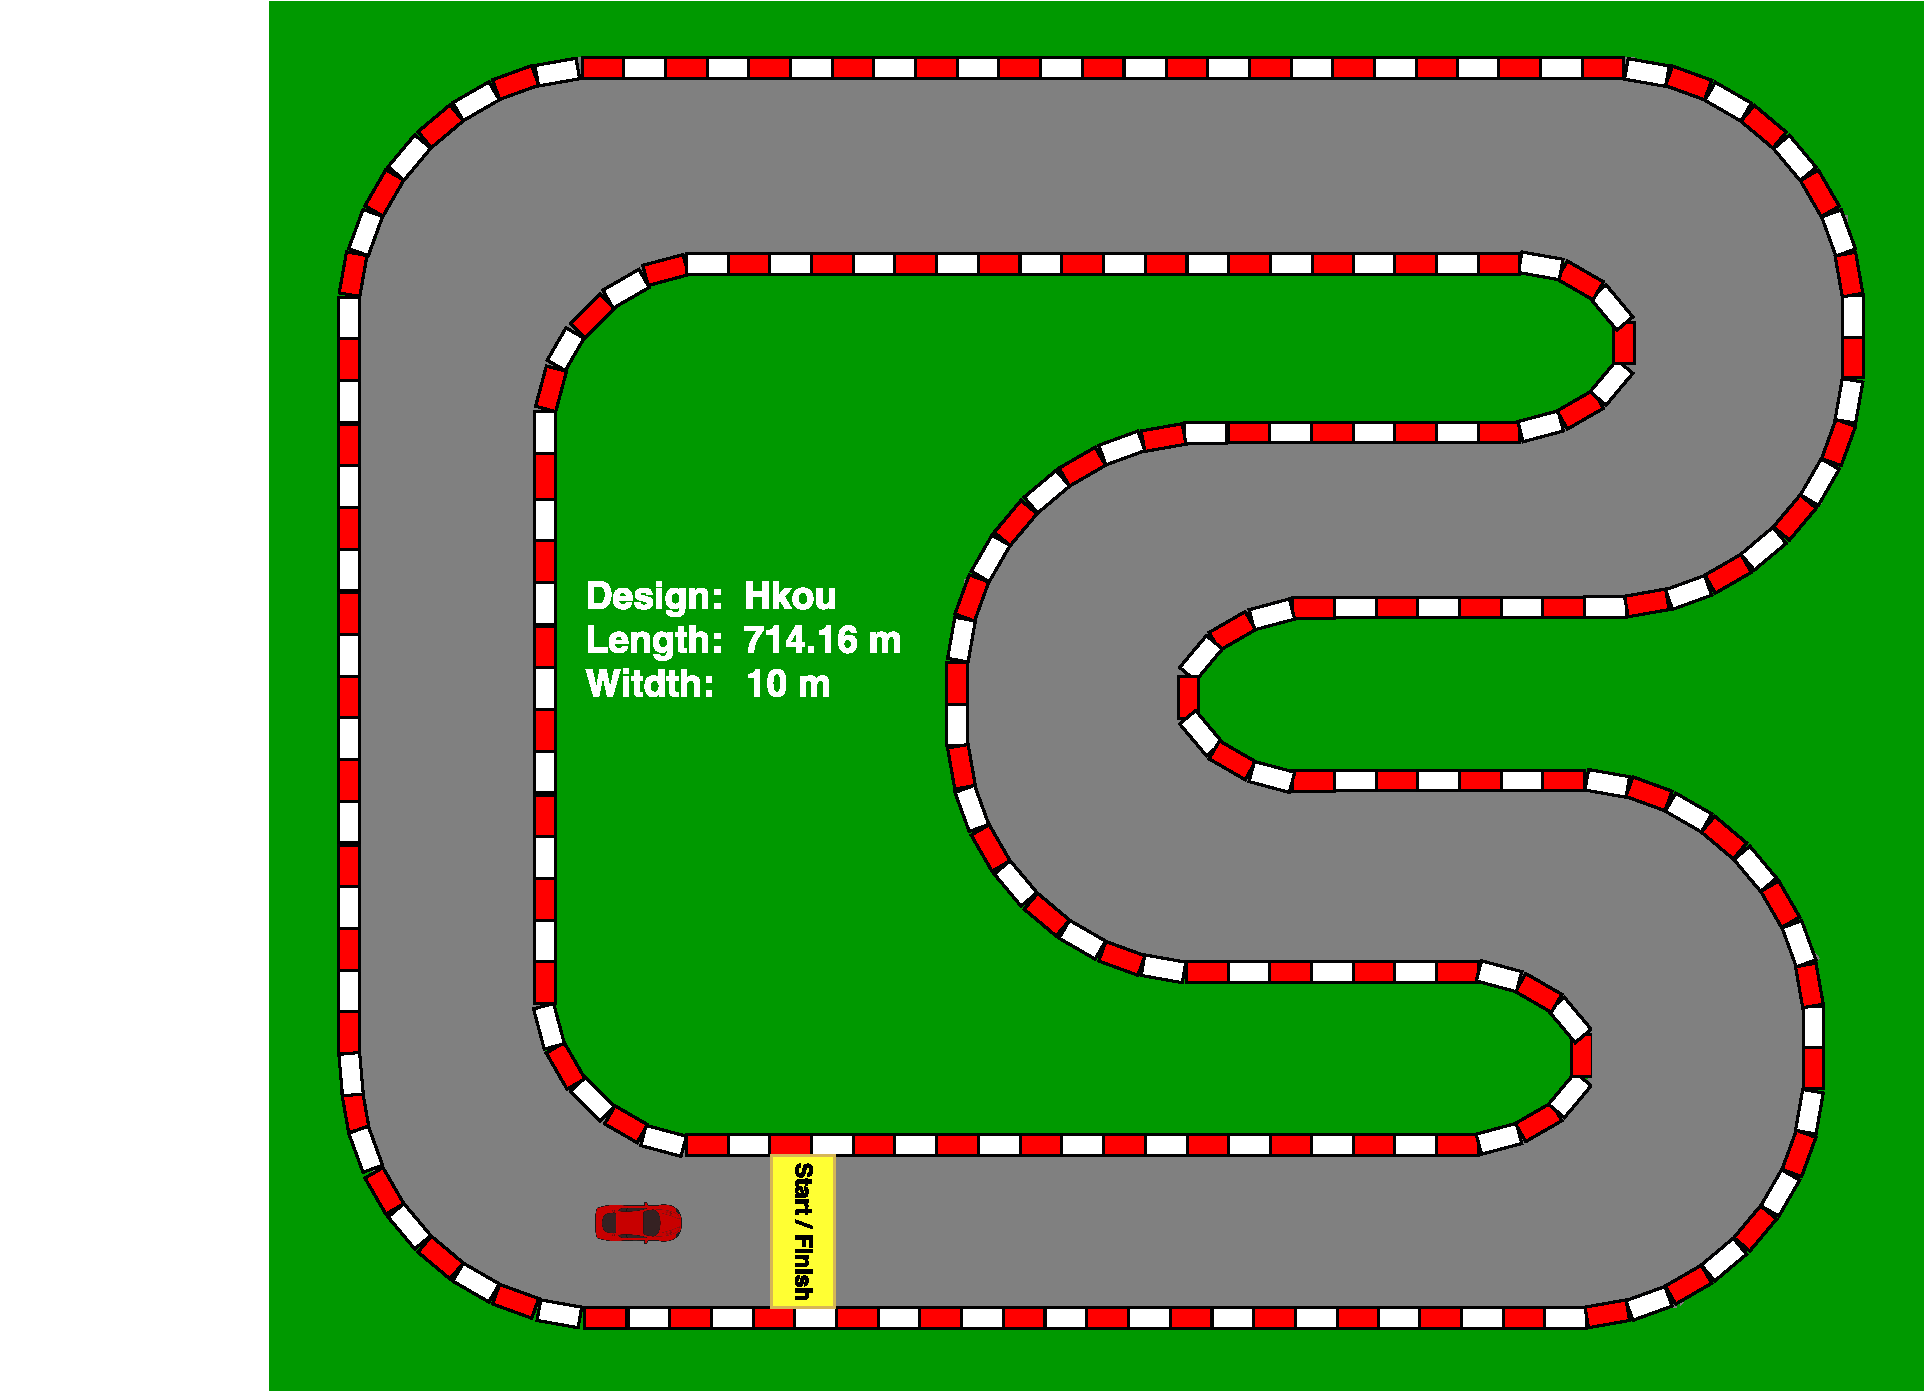
\includegraphics[width=1\textwidth]{Figures/Result/track_simple_1.pdf}
	\caption{The first track used is called $simple\_1$ made by Hkou}
	\label{fig:track_simple_1}
\end{figure}

To find other tracks to train and test on, it has to look similar to the one on \Cref{fig:track_simple_1}, because as mentioned before it learns from the input image. So if it should be possible to test the trained agent, it has to see some of the same things on the test track as on the training track. In the TORCS environment there are three tracks, which look similar the one on \Cref{fig:track_simple_1} and two others. 

The second track used in this project is a track which looks really similar to the first track, and the name is simple\_2 instead of simple\_1. The only difference from the first track is, it is mirrored. This mean that all the turns are exactly opposite. The track is thereby good for testing, because it has different turns than the first track. The second track can be seen on \Cref{fig:track_simple_2}.

\begin{figure}[H]
	\centering
	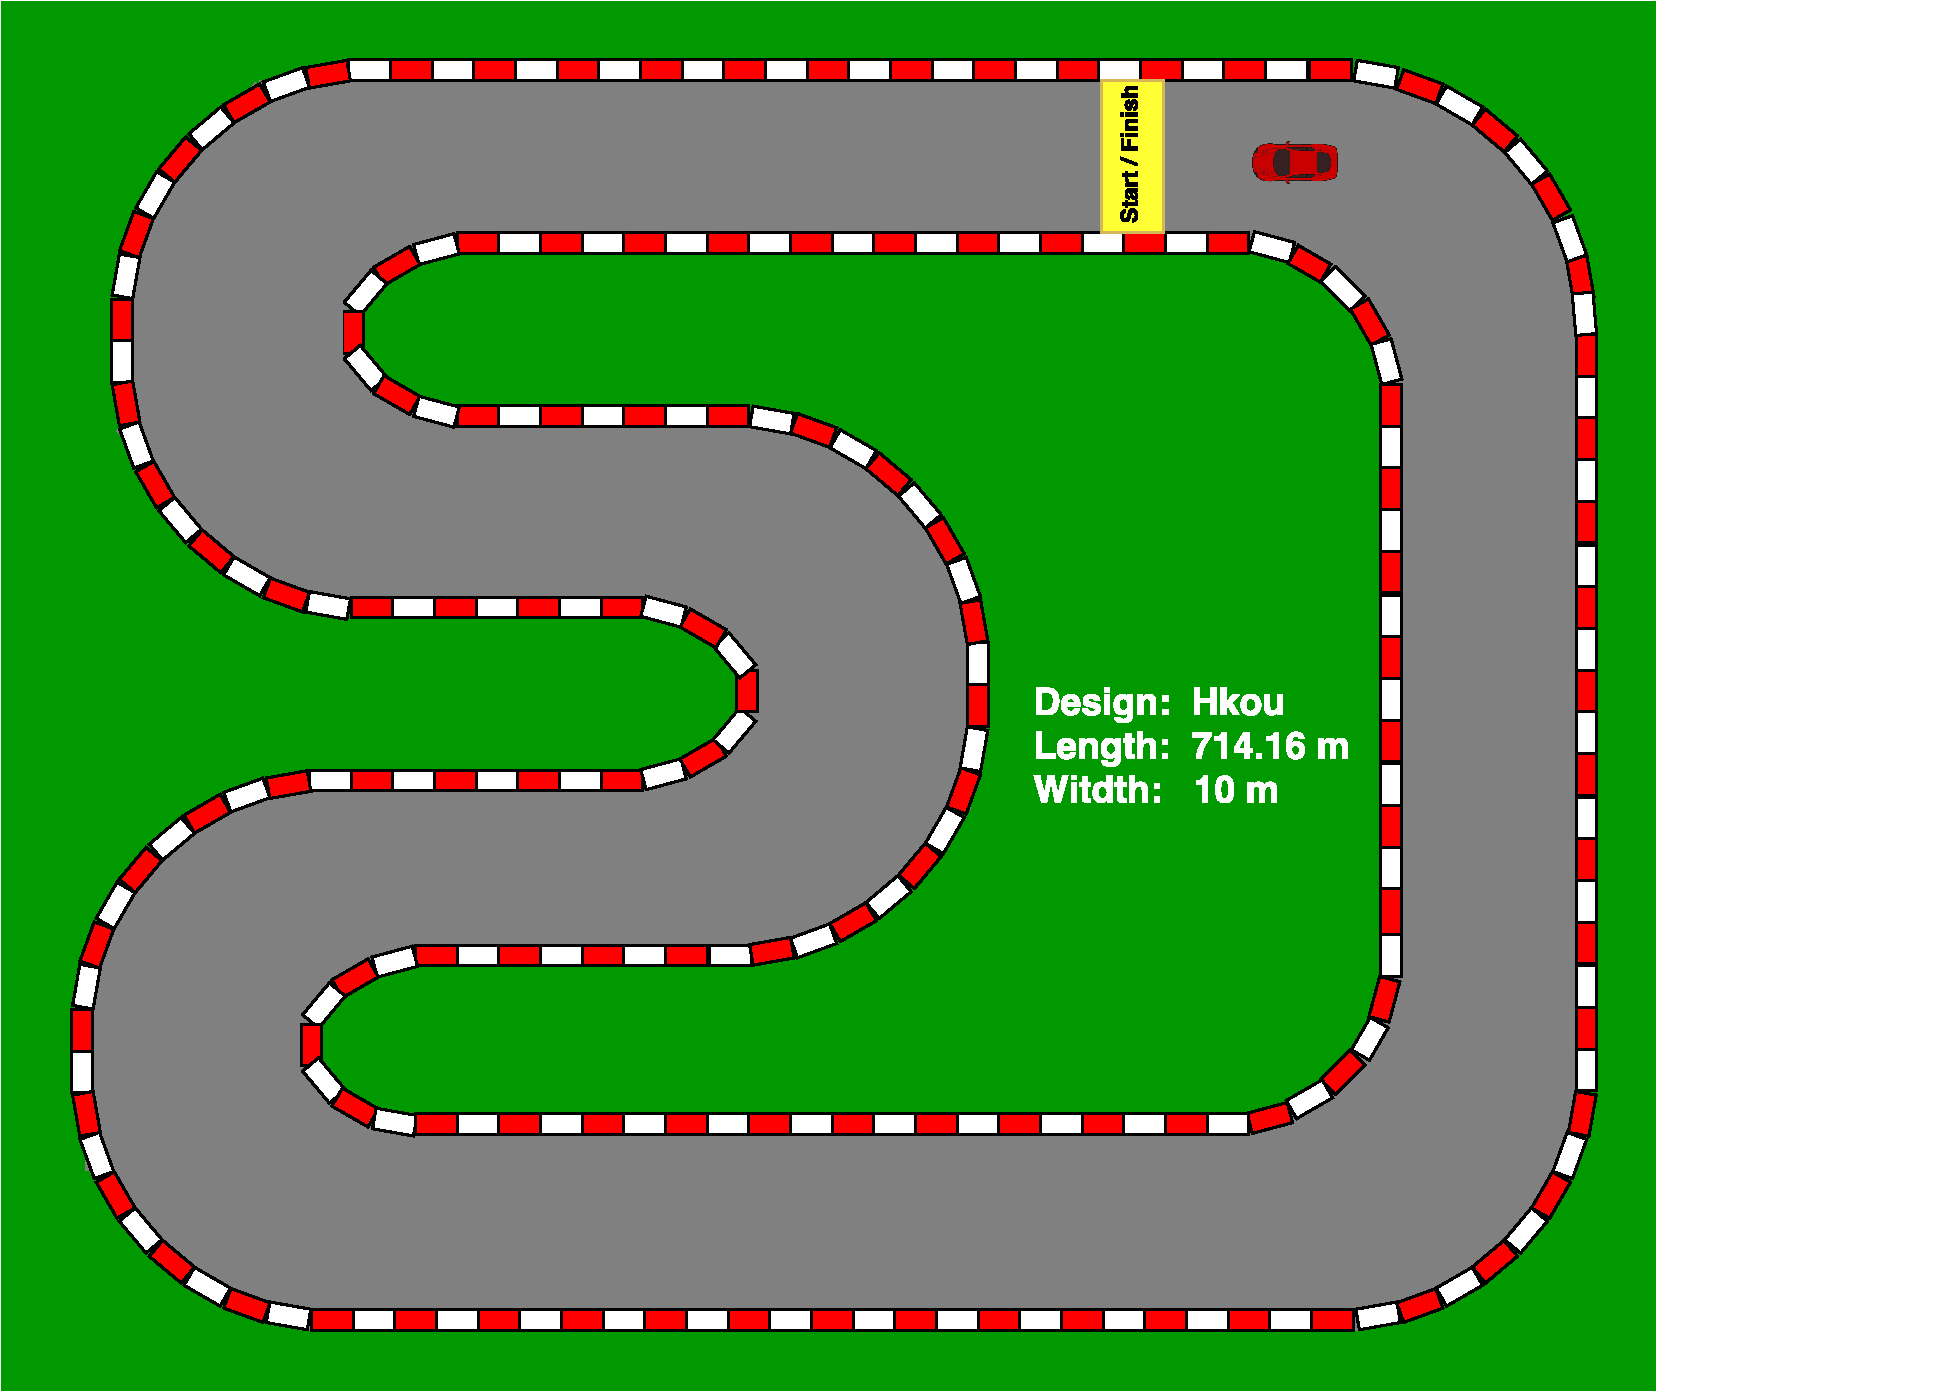
\includegraphics[width=1\textwidth]{Figures/Result/track_simple_2.pdf}
	\caption{The second track used is called $simple\_2$ made by Hkou}
	\label{fig:track_simple_2}
\end{figure}

The last track is similar to the two other tracks on \Cref{fig:track_simple_1} and \Cref{fig:track_simple_2}. The only difference is it is more simple, only has left turns. Another difference form the other two tracks is the length it is much longer than the other tracks. It is because of this length it is used to see how the agent learns on a different track with a longer distance. The last used track in this project can be seen on \Cref{fig:track_longstr}. 

\begin{figure}[H]
	\centering
	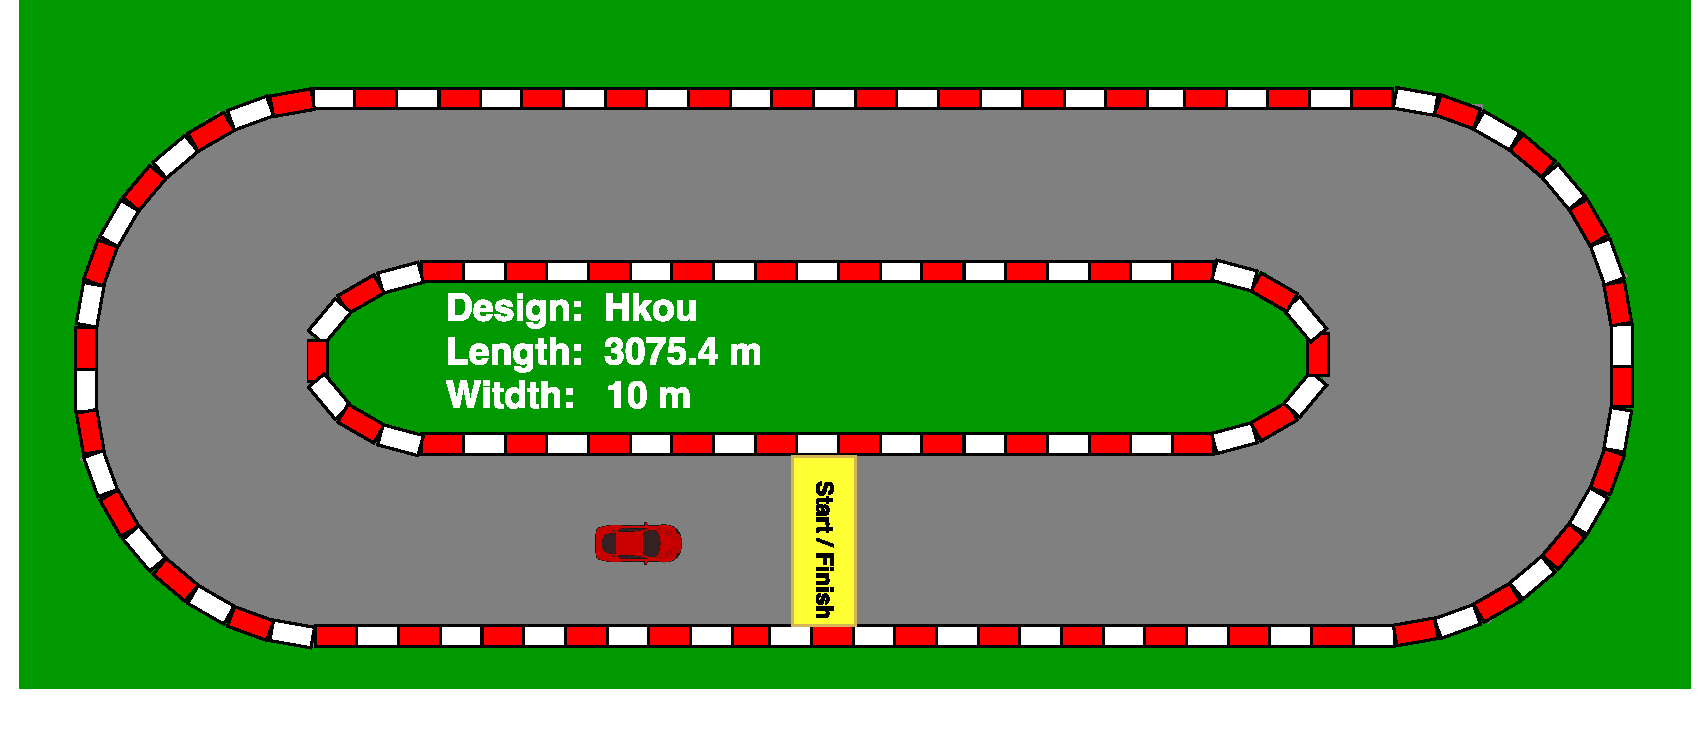
\includegraphics[width=1\textwidth]{Figures/Result/track_longstr.pdf}
	\caption{The third track used is called $longstr$ made by Hkou}
	\label{fig:track_longstr}
\end{figure}


\subsection*{Training}
In this project, it is tested if the tracks has an influence on the training. This is done to see if there is some of the used track which is better to train on than others.

To compare this training the reward graph is used, the agent has trained on the three different tracks (\Cref{fig:track_simple_1}, \Cref{fig:track_simple_2} and \Cref{fig:track_longstr}). Here it would be better if the reward is growing faster on one of the tracks than the others, and even more important converge to the optimal reward faster. The reward graph can be seen on \Cref{fig:change_of_track_reward_graph}.

\begin{figure}[H]
	\centering
	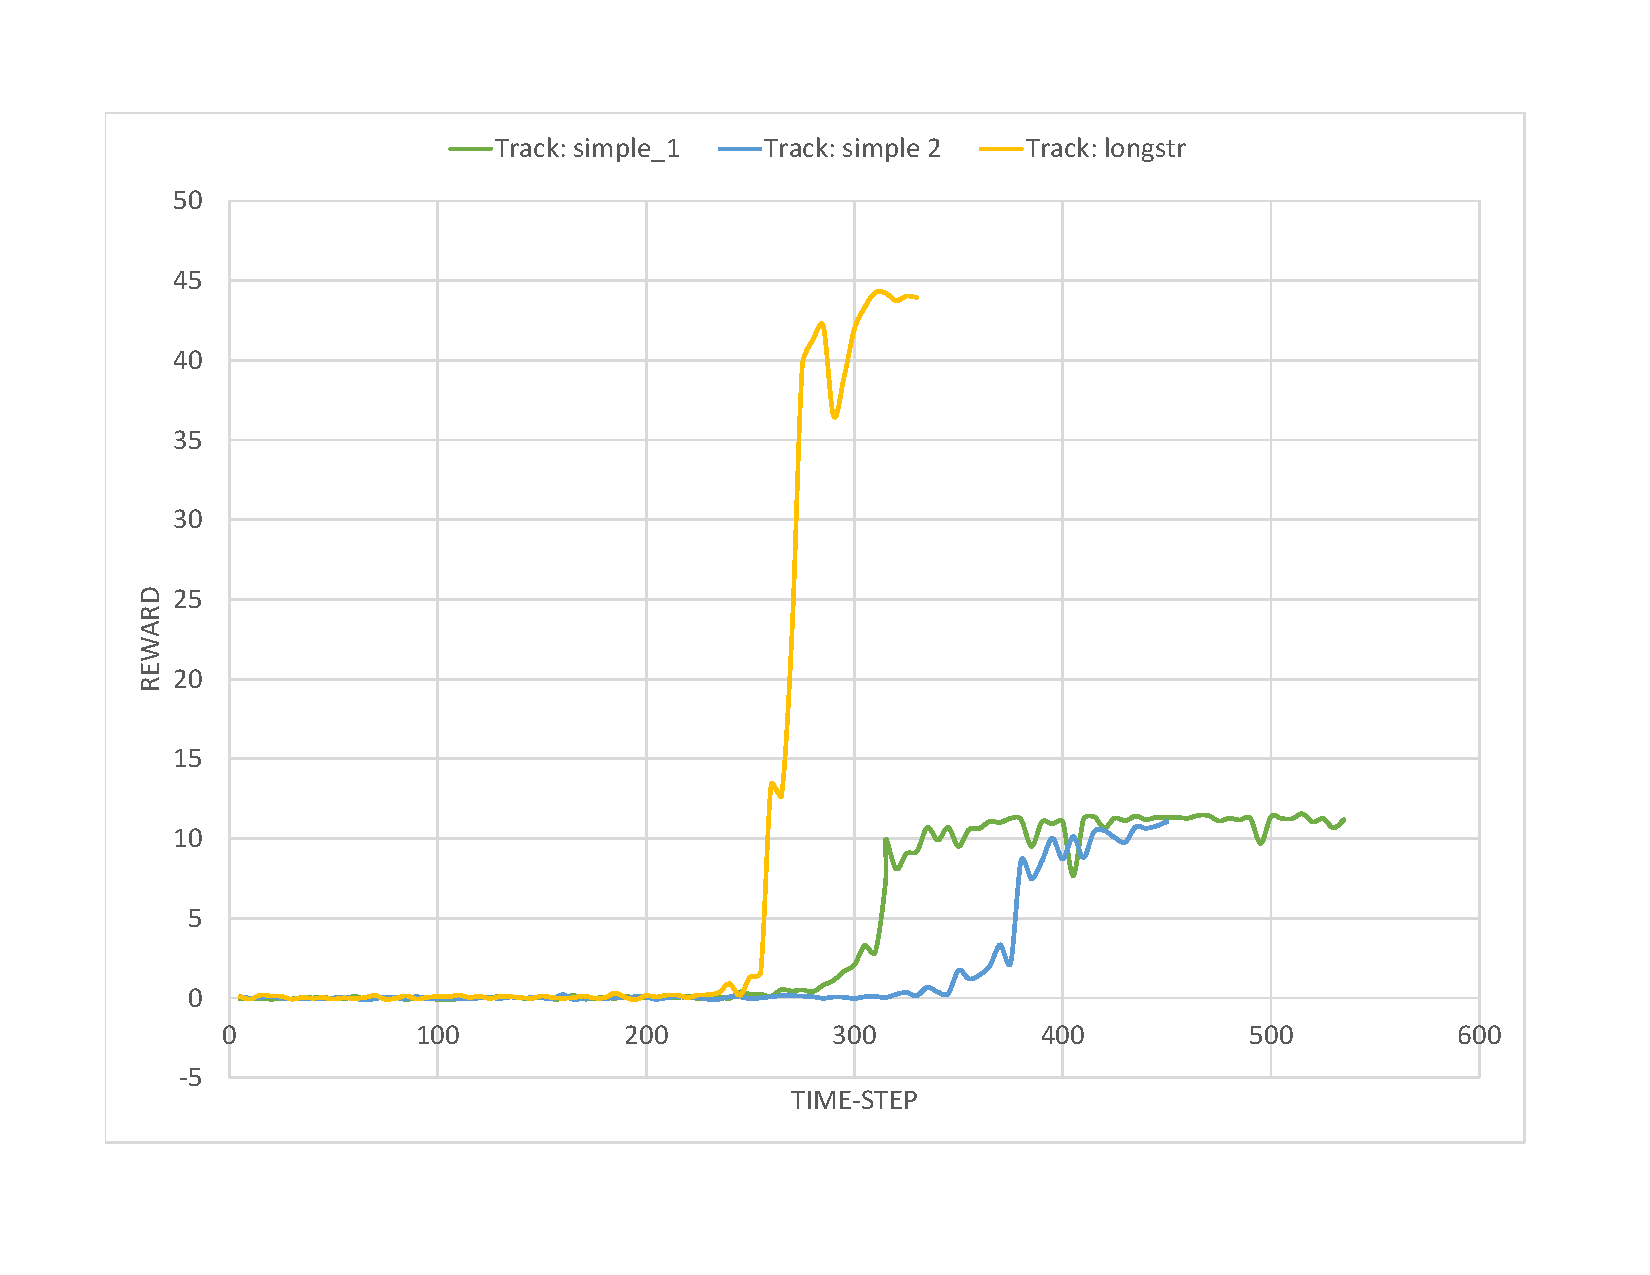
\includegraphics[width=1\textwidth]{Figures/Result/change_of_track_reward_graph.pdf}
	\caption{Comparison of the three different tracks with the reward getting from the environment}
	\label{fig:change_of_track_reward_graph}
\end{figure}

As seen on \Cref{fig:change_of_track_reward_graph} the different track have a small influence on when the reward starts learning. The track longstr learns around 270 time-steps, simple\_1 around 320 time-steps and simple\_2 around 370 time-steps. Here it is hard to say why it learns faster on the simple\_1 track than the simple\_2, because it is the same track just mirrored. It could be the decision taking on the simple\_1 track is better than the one on simple\_2, so another training would then maybe vary a bit. Here it also seems to learn the track longstr faster, this could be because it is simpler than the other tracks.  

The difference is the reward on the third track, which can be seen to converge to a bigger reward 43, than the reward from the two other tracks 11. This is because of the length of the track. It can get a bigger reward, when the track is longer. The reward is given by every step and added together to a total reward, this means if there is more steps, then the total reward is bigger. Another way to look at it is the length of every time-step is longer. The length of the episodes on the different tracks can be seen on \Cref{fig:change_of_track_length_graph }     

\begin{figure}[H]
	\centering
	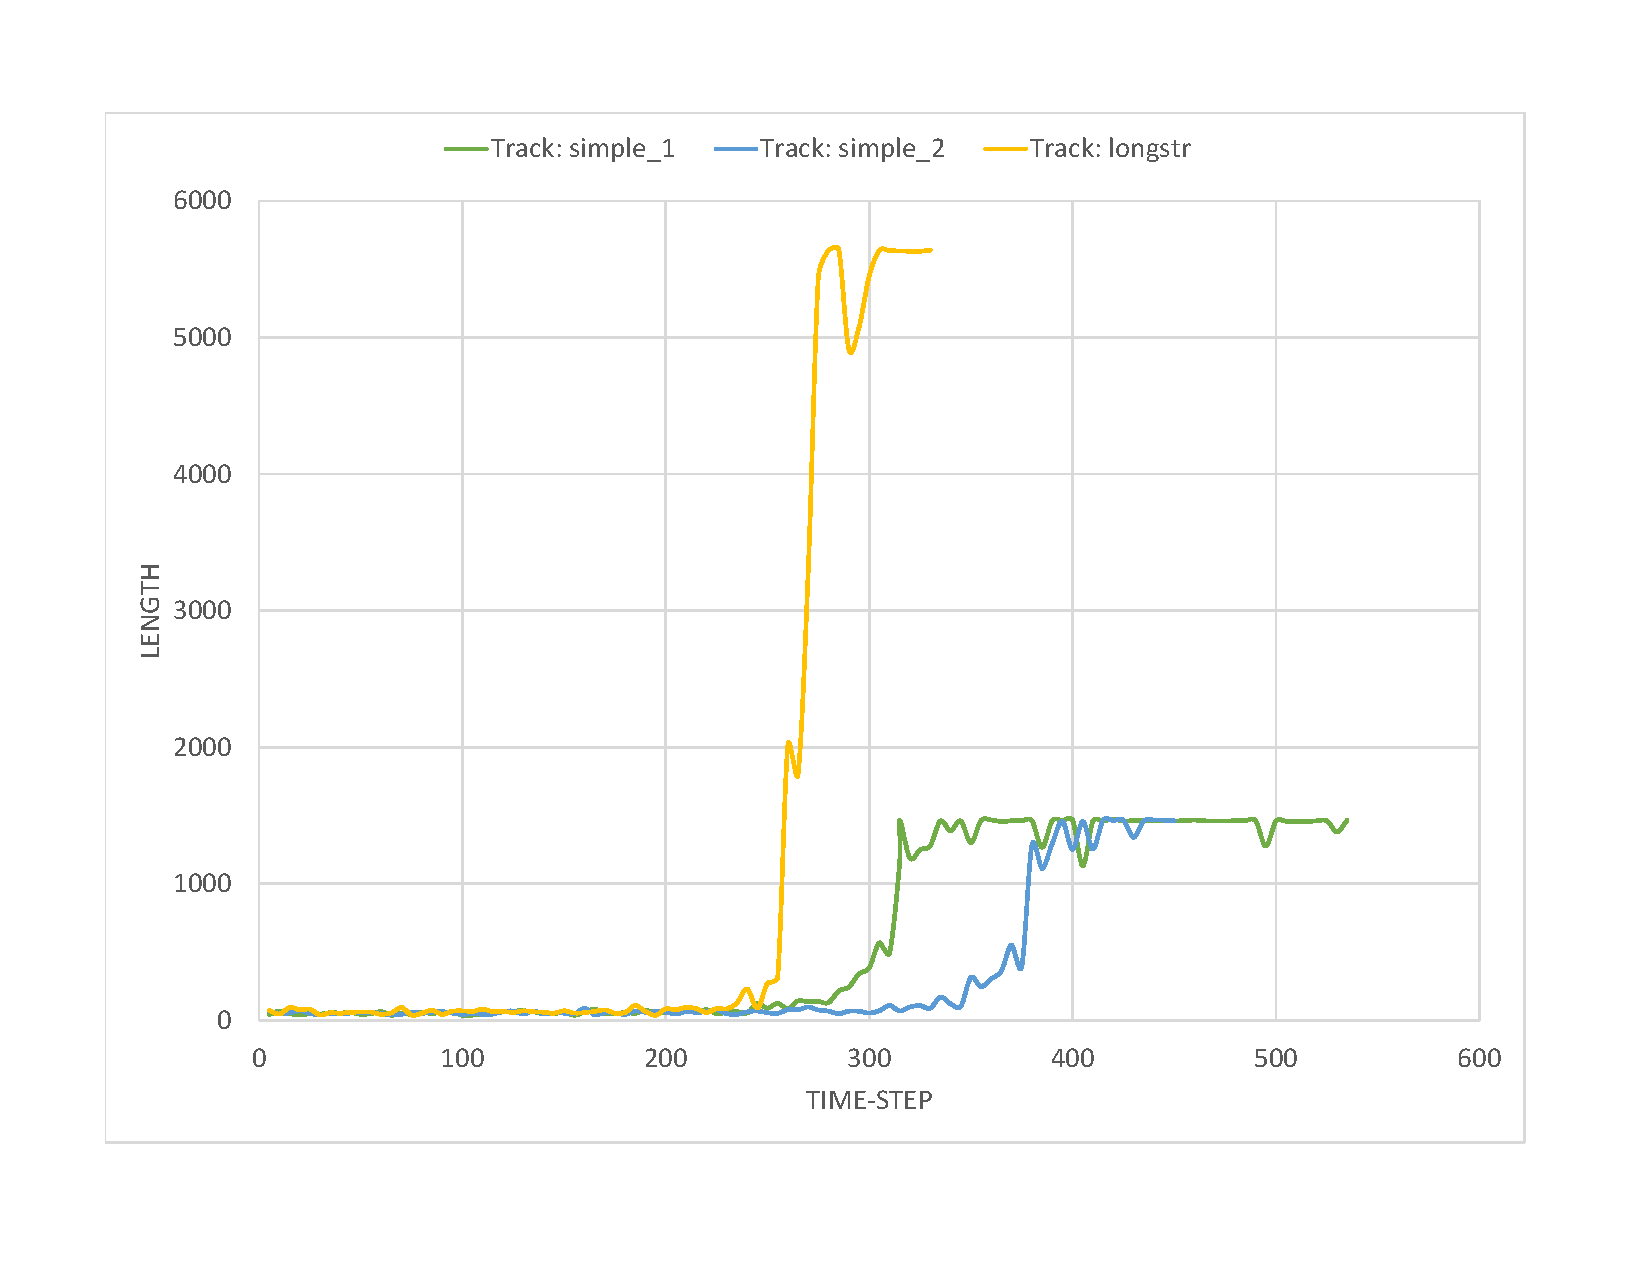
\includegraphics[width=1\textwidth]{Figures/Result/change_of_track_length_graph.pdf}
	\caption{Comparison of the three different tracks with the length of the episodes}
	\label{fig:change_of_track_length_graph}
\end{figure}

Because the track is 3-4 times longer the reward is also 3-4 times bigger:
\begin{equation}
\frac{\mathrm{Length \ of \ longstr}}{\mathrm{Length \ of \ simple\_1}} = \mathrm{Length \ difference}   \qquad \rightarrow \qquad \frac{3075.4}{714.16} = 4.31  
\end{equation}
\begin{equation}
\frac{\mathrm{Reward \ of \ longstr}}{\mathrm{Reward \ of \ simple\_1}} = \mathrm{Reward \ difference}   \qquad \rightarrow \qquad \frac{44}{11} = 4
\end{equation}
By looking of the result of the two equations, it looks like the bigger reward is just the difference of the length of the tracks. 


After these result the track which have been used in all the other trainings is the first track seen on \Cref{fig:track_simple_1}. To test if the agent has learned how to drive the second track is used seen on \Cref{fig:track_simple_2}. If the agent is able to complete a lap on both of these tracks it is concluded the agent has learned how to drive.   



